% ---------------------------------------------------------------------------
% Präambel für BHT-Abgaben. Unverändert übernehmen.
% Gebaut mit: tectonic datei.tex
% ---------------------------------------------------------------------------
\documentclass[11pt,a4paper,oneside]{article}

\usepackage[ngerman]{babel}
\usepackage{lmodern}
\usepackage{geometry}
\usepackage{fancyhdr}
\usepackage{booktabs}
\usepackage{array}
\usepackage{tabularx}
\usepackage{float}
\usepackage{graphicx}
\usepackage[htt]{hyphenat}
\usepackage[hidelinks]{hyperref}
\usepackage{xurl}

\geometry{left=3cm, right=2.5cm, top=2.5cm, bottom=2.5cm}
\sloppy
\emergencystretch=3em
\newcolumntype{L}{>{\raggedright\arraybackslash}X}

\pagestyle{fancy}
\fancyhf{}
\lhead{\small Mobile Geoanwendungen -- Sommersemester 2026}
\rhead{\small Kurzbeschreibung: Kaskade}
\cfoot{\thepage}
\renewcommand{\headrulewidth}{0.4pt}

\begin{document}

\begin{center}
{\normalsize BERLINER HOCHSCHULE FÜR TECHNIK}\\[0.2em]
{\small MOBILE GEOANWENDUNGEN, Sommersemester 2026}\\[1.4em]
{\LARGE\textbf{Kaskade}}\\[0.4em]
{\large Kurzbeschreibung}\\[1.2em]
Carl Janek Markert (Matrikelnummer 105906)\\
Paul Tschätsch (Matrikelnummer 107359)\\[0.6em]
22.~September 2026
\end{center}

\vspace{1.5em}

\section*{Worum es geht}

Kaskade ist eine native iOS-App, die vier Ortungsverfahren -- GNSS,
Ultrabreitband (UWB), Bluetooth-RSSI (BLE) und LiDAR -- nach demselben
Protokoll gegen einen unabhängigen Referenzwert vermisst: Sollwert,
Aufzeichnung, CSV-Export, Auswertung. Als Anwendungsfall, der diese
Ortungskaskade motiviert, klassifiziert die App zusätzlich den
Transportmodus einer Fahrt über ein selbst trainiertes Modell (Fuß, Rad,
Auto, Zug) -- eine Unterscheidung, die Apples Systemklassifikator
\texttt{CMMotionActivity} strukturell nicht leisten kann.

Vier Messstudien mit echten Felddaten: GNSS-Genauigkeit an drei
ALKIS-Referenzpunkten (M1), Transportmodus-Klassifikation gegen die
Systembaseline (M2), UWB gegen BLE im Nahbereich (M3) und LiDAR gegen ein
Maßband (M4). M1, M3 und M4 belegen die vier Ortungsverfahren, M2 prüft den
Anwendungsfall. Details, Zahlen und Grafiken stehen im vollständigen
Abgabedokument \texttt{abgabe.pdf}.

\section*{Technologien}

\begin{table}[H]
\centering
\small
\begin{tabularx}{\linewidth}{@{}lL@{}}
\toprule
\textbf{Bereich} & \textbf{Technologie} \\
\midrule
Positionierung & CoreLocation (GNSS), ausgewertet gegen ALKIS-Referenzpunkte \\
Nahbereichsortung & NearbyInteraction (UWB), CoreBluetooth/CLBeaconRegion (BLE-RSSI) \\
Nahfeldmessung & ARKit \texttt{sceneDepth} (LiDAR) \\
Klassifikation & scikit-learn Random Forest, exportiert über coremltools nach Core~ML \\
Karten & MapLibre GL (iOS-App und Native), MapLibre GL JS (Standalone-Viewer) \\
Speicherung & SQLite über GRDB, CSV-/GeoJSON-Export \\
Plattform & Natives SwiftUI, iOS~17+ \\
\bottomrule
\end{tabularx}
\end{table}

\section*{Aufbau des Repositories}

\begin{description}
    \item[\texttt{ios/}] SwiftUI-App (Xcode-Projekt aus \texttt{project.yml} über XcodeGen erzeugt)
    \item[\texttt{analysis/}] Python-Training und -Auswertung, \texttt{run\_all.py} erzeugt alle Abbildungen/Tabellen neu
    \item[\texttt{data/}] eingecheckte Rohmessreihen, Tracks und Referenzpunkte
    \item[\texttt{viewer/}] eigenständiger Betrachter für exportierte Feldtest-Tracks (MapLibre GL JS)
    \item[\texttt{docs/abgabe/}] vollständiges Abgabedokument
\end{description}

\section*{Screenshots}

\begin{figure}[H]
\centering
\raisebox{-\height}{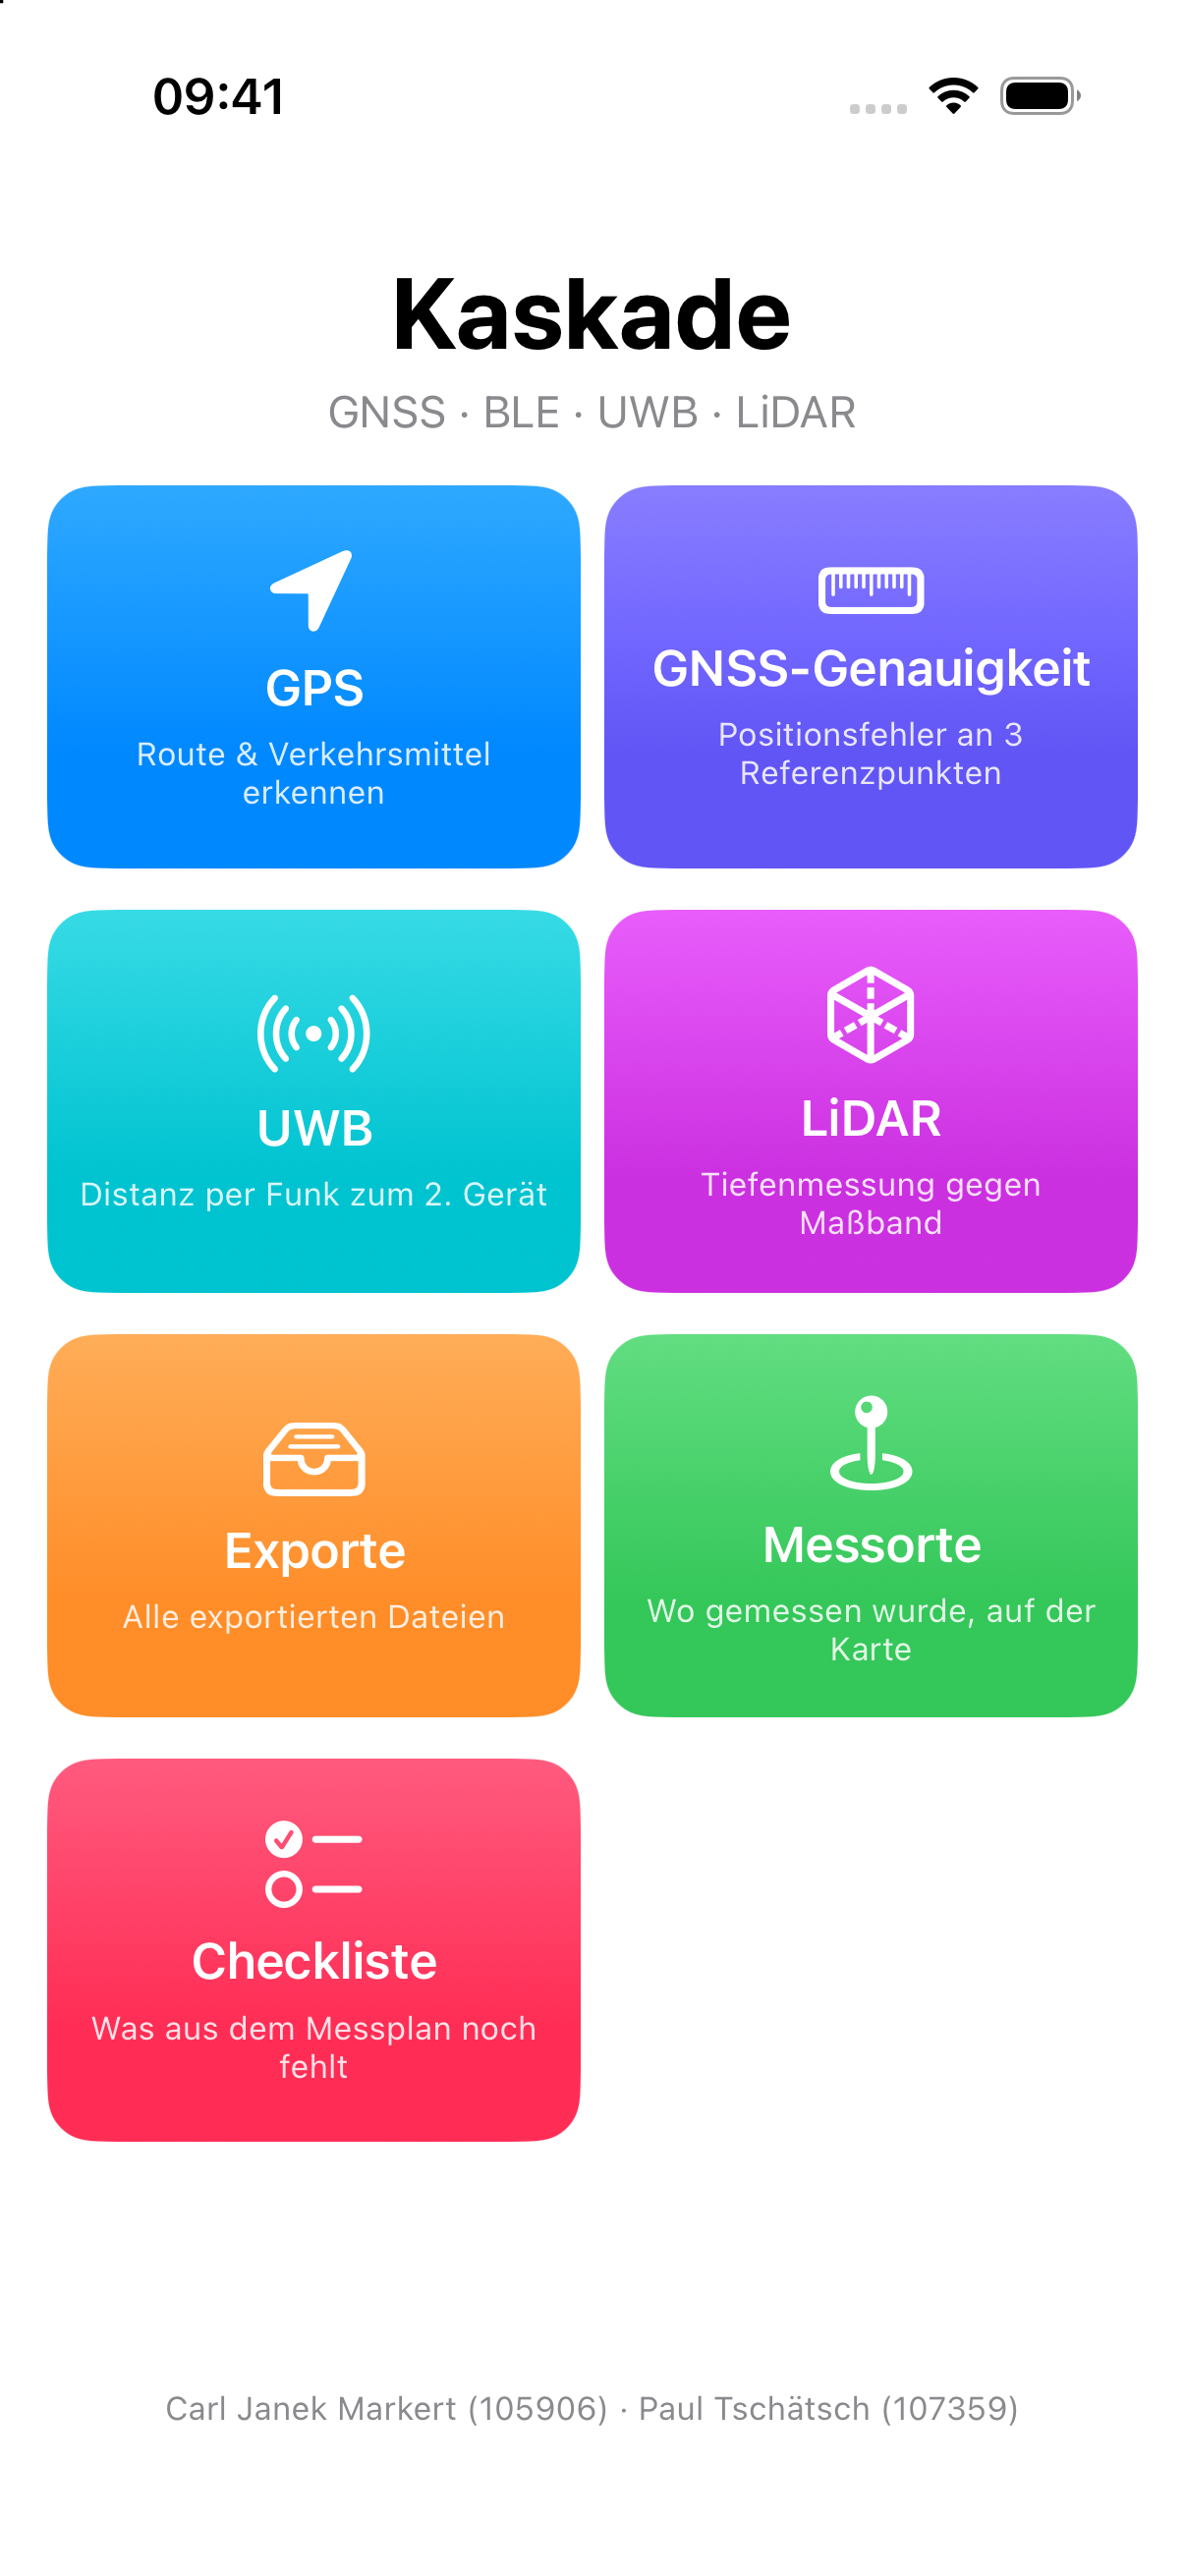
\includegraphics[width=0.23\linewidth]{../../4_proof_of_concept/screenshot_startbildschirm.png}}\hfill
\raisebox{-\height}{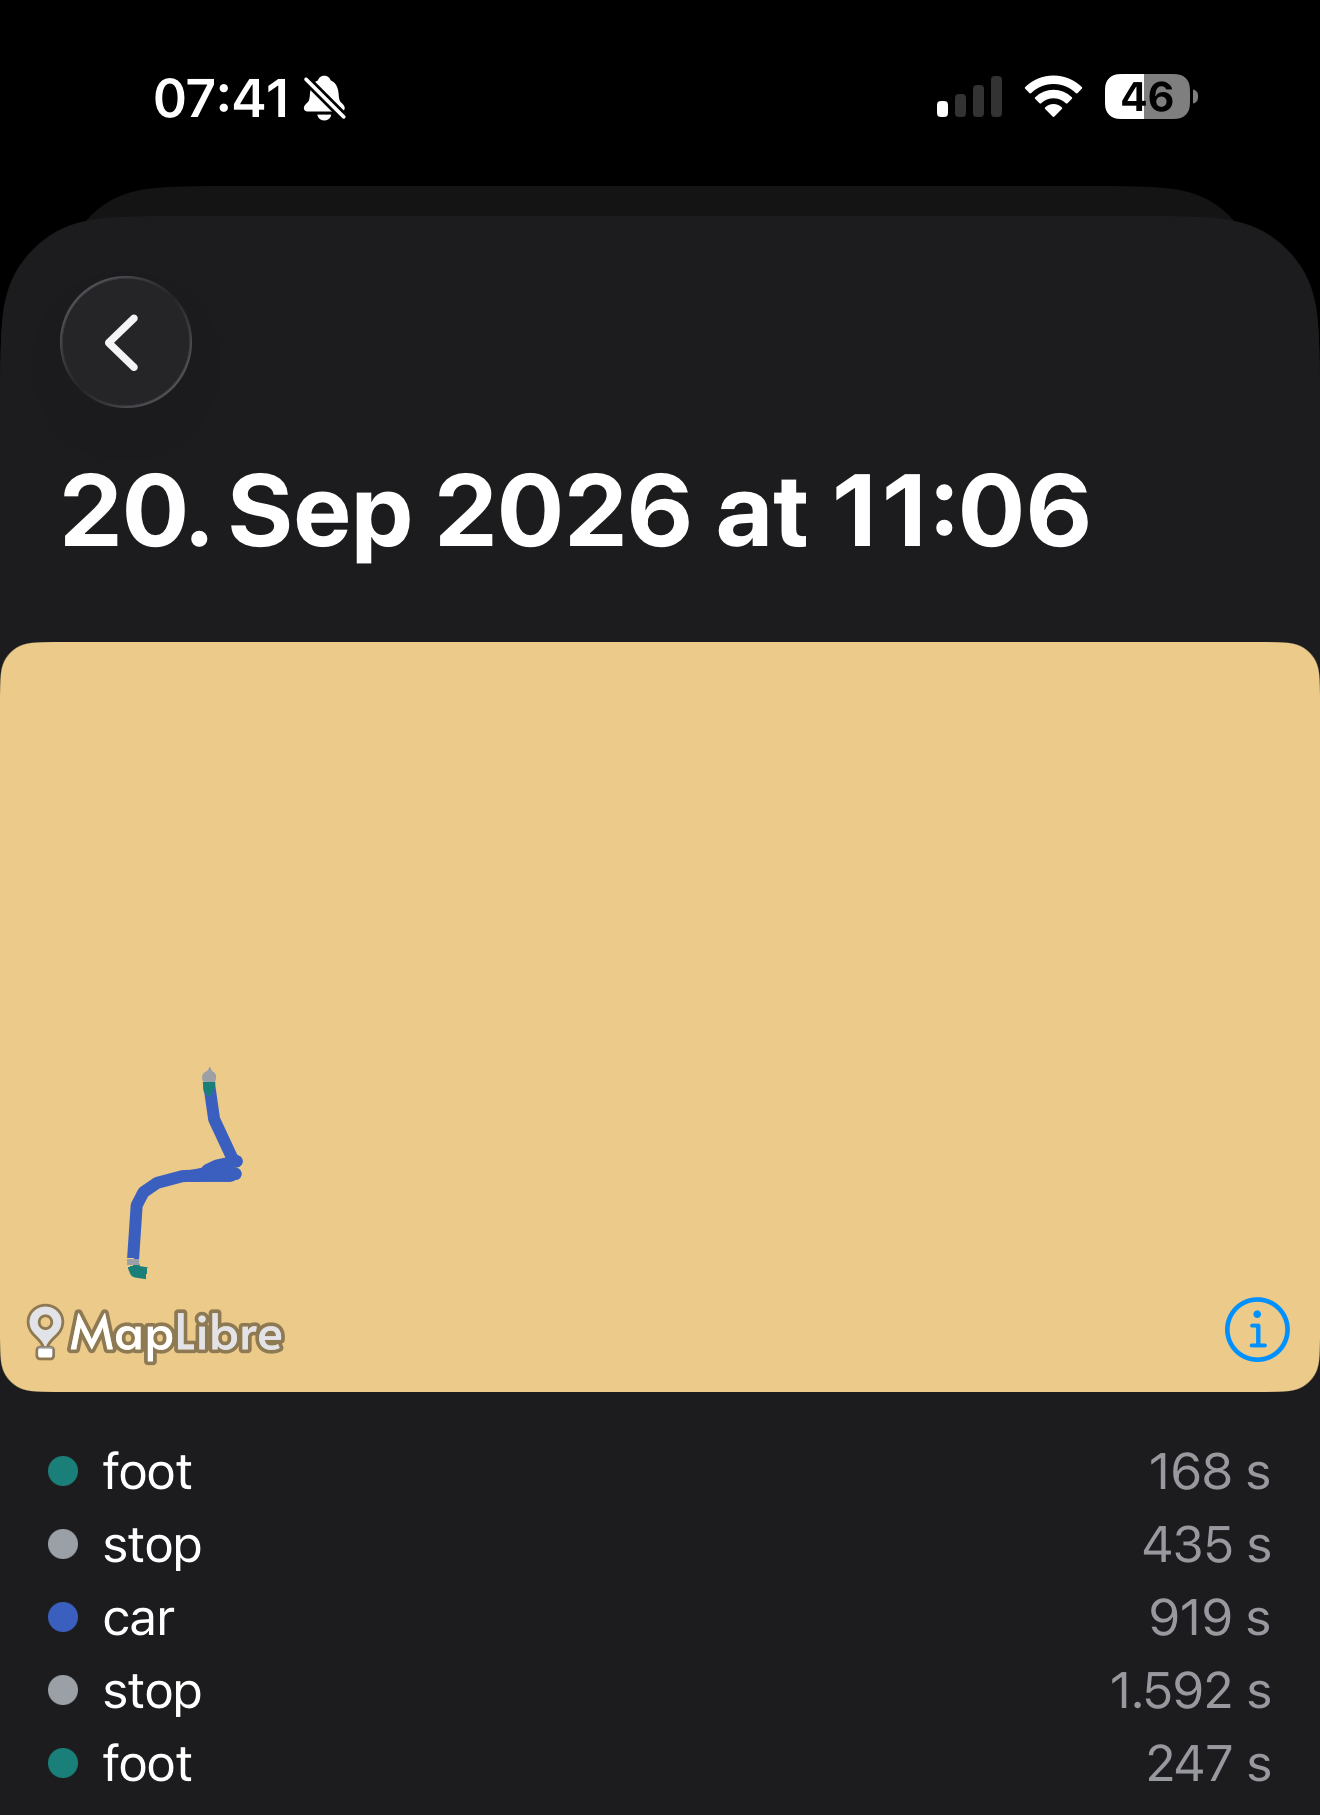
\includegraphics[width=0.23\linewidth]{../../4_proof_of_concept/screenshot_trip_segmente.png}}\hfill
\raisebox{-\height}{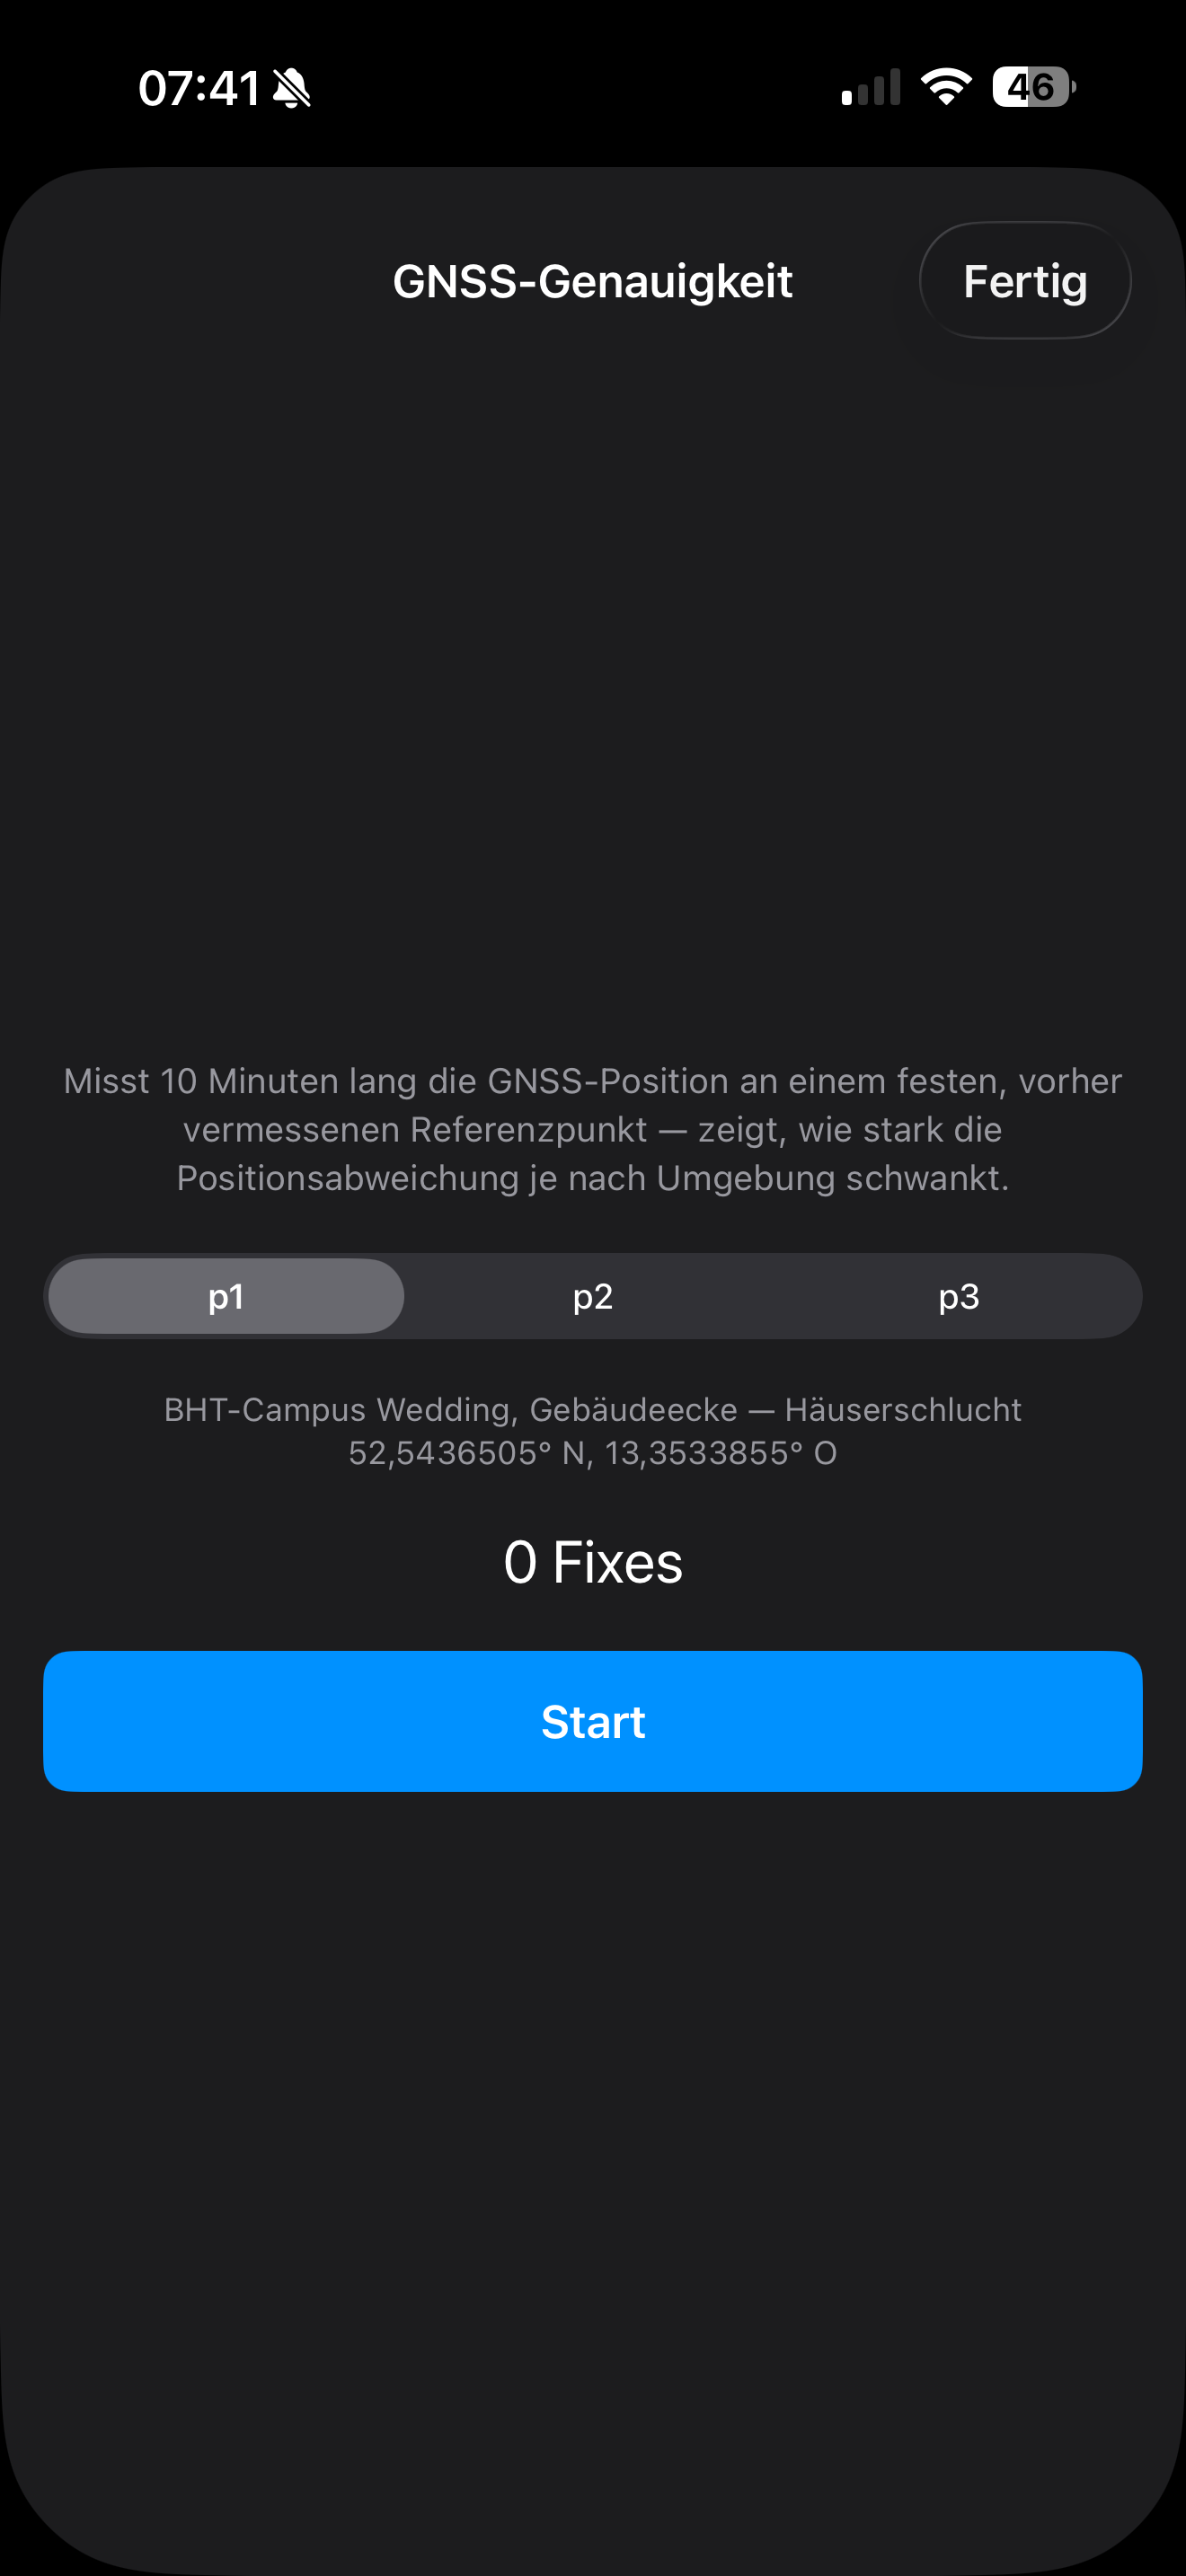
\includegraphics[width=0.23\linewidth]{../../4_proof_of_concept/screenshot_m1_gnss.png}}
\caption{Links: Startbildschirm mit den sieben Werkzeugen für Aufzeichnung,
Messstudien und Export. Mitte: Trip vom 20.09. mit Karte und
Segmentierung in Fußwege, Stopps und Fahrt (Handlabels \texttt{foot} und
\texttt{car}). Rechts: M1, GNSS-Genauigkeit am Referenzpunkt~p1 (BHT-Campus
Wedding, Häuserschlucht), zehn Minuten Messdauer.}
\end{figure}

\begin{figure}[H]
\centering
\raisebox{-\height}{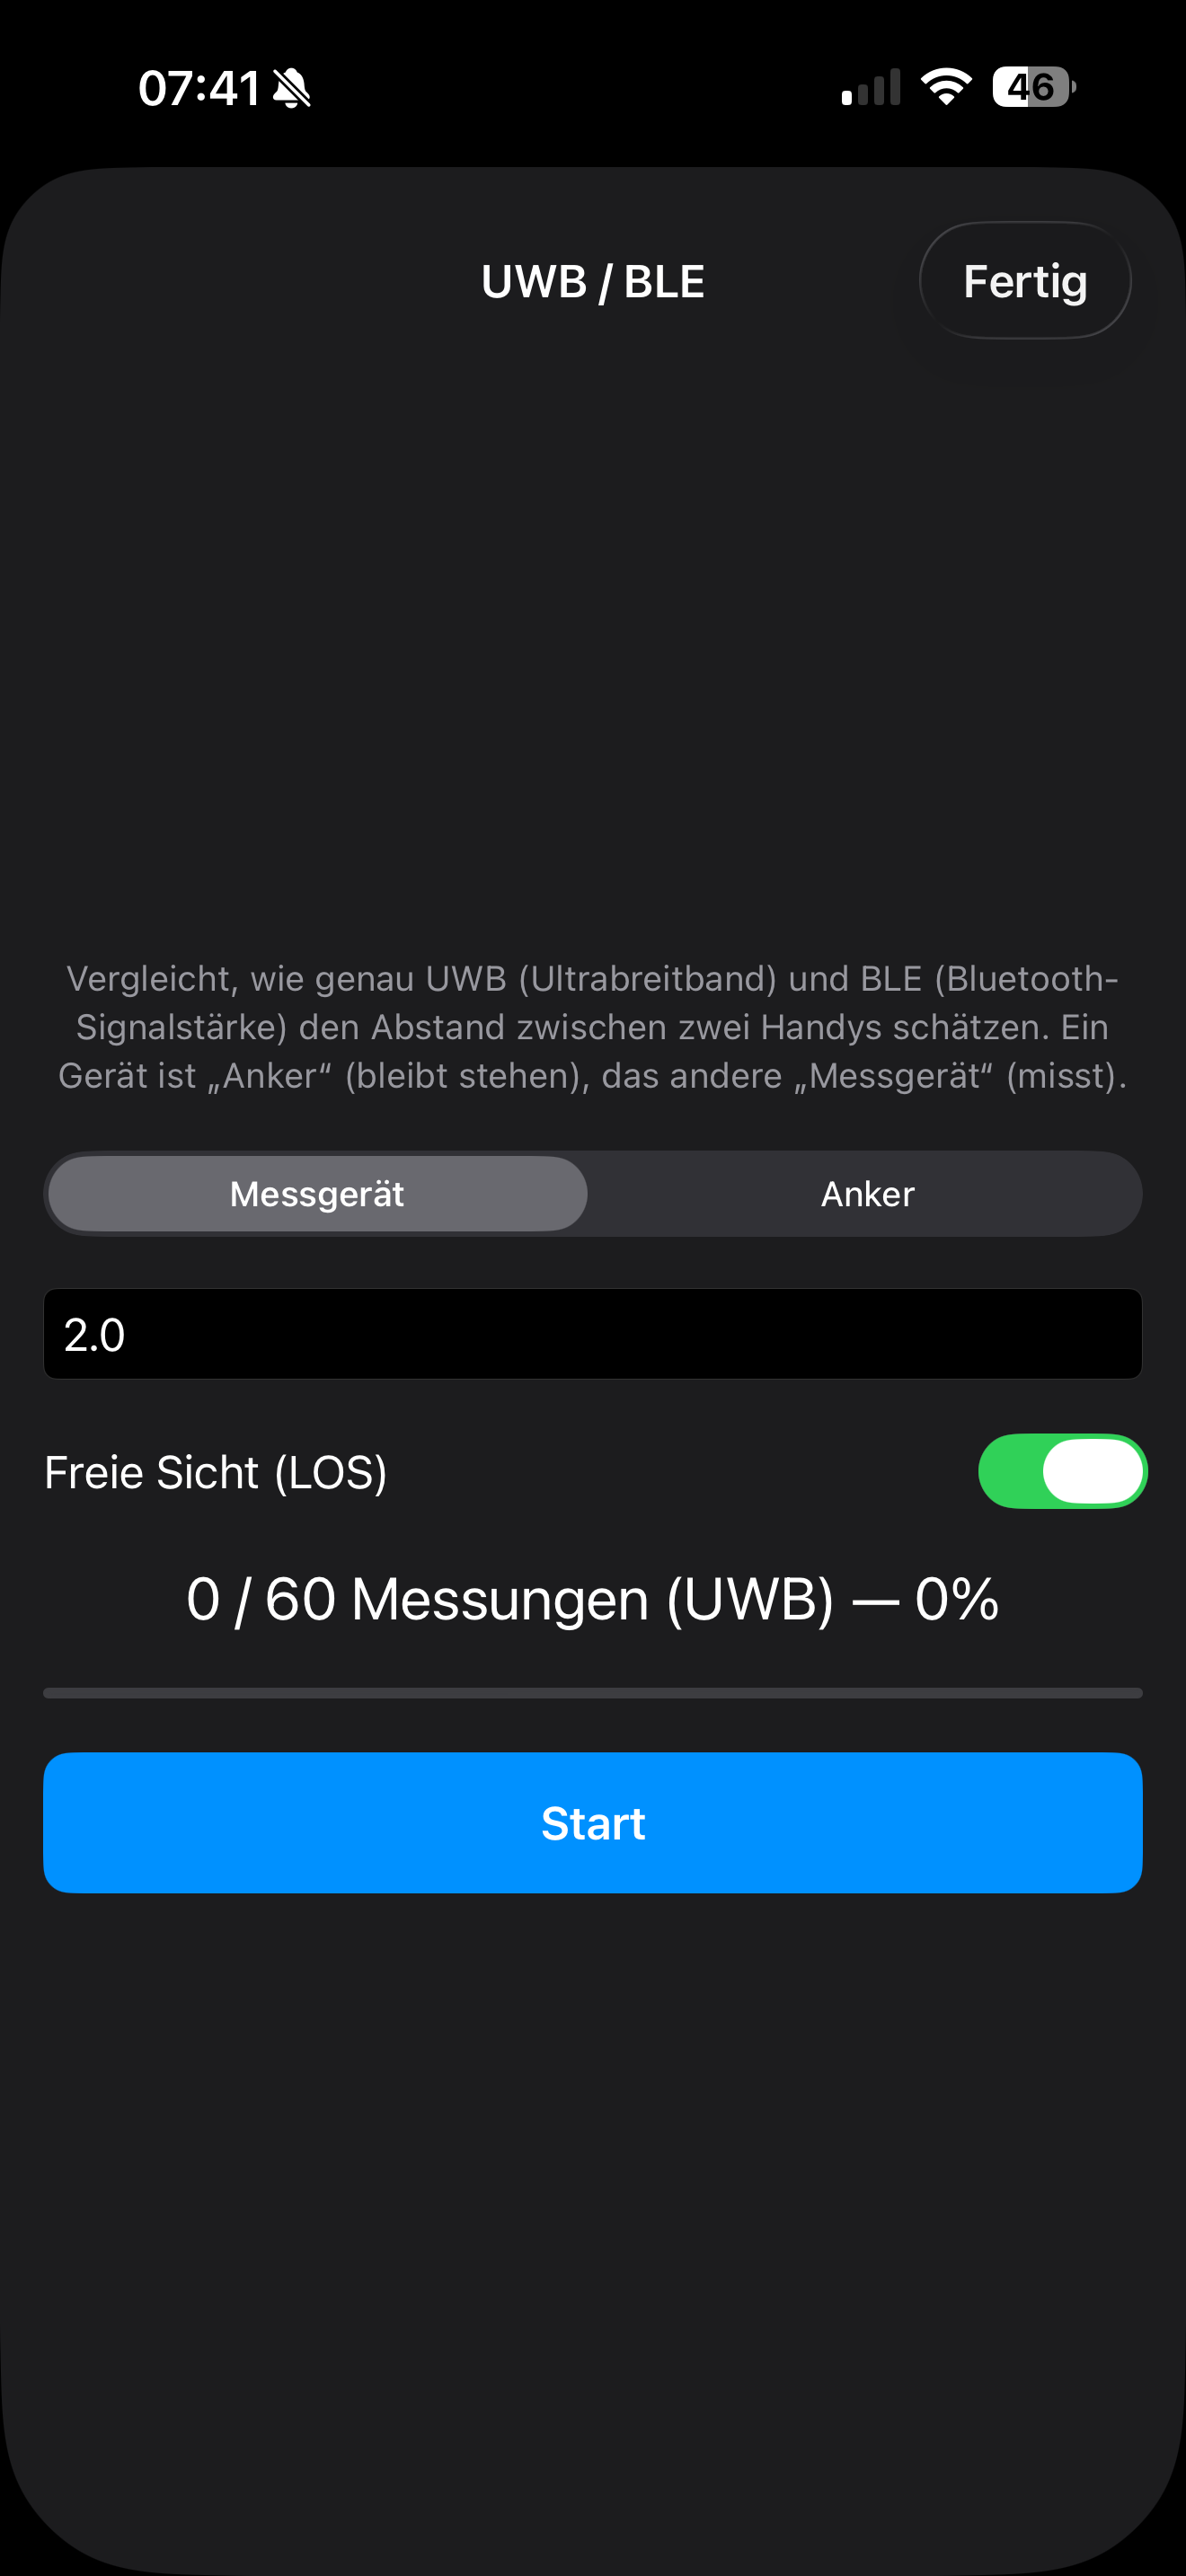
\includegraphics[width=0.23\linewidth]{../../4_proof_of_concept/screenshot_m3_uwb_ble.png}}\hspace{1.2cm}
\raisebox{-\height}{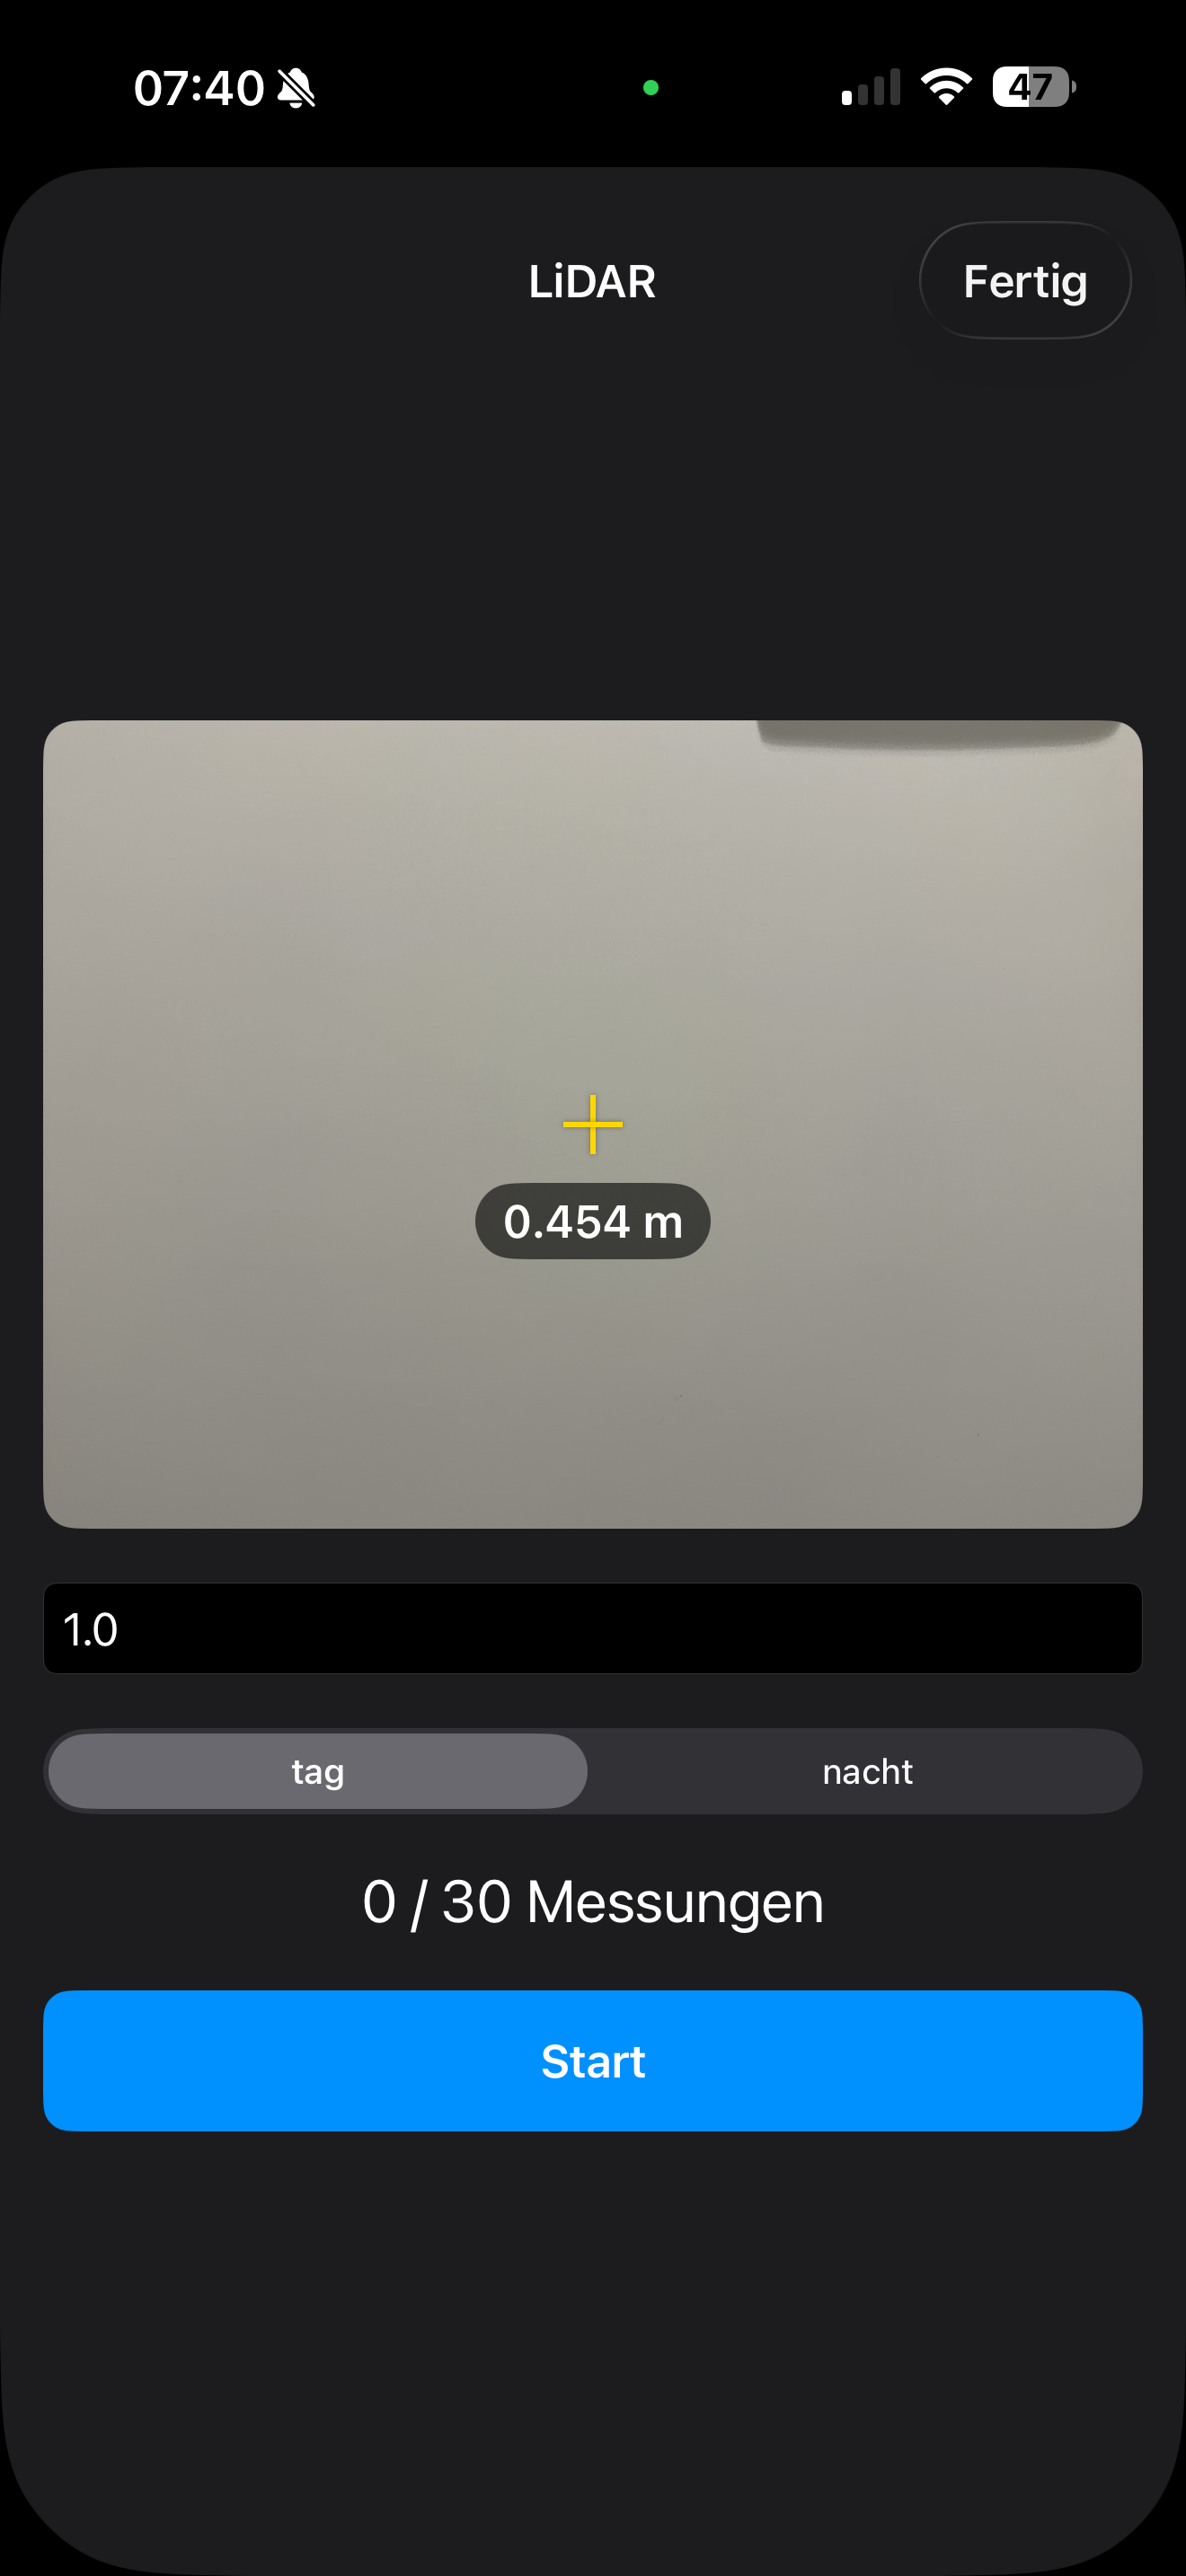
\includegraphics[width=0.23\linewidth]{../../4_proof_of_concept/screenshot_m4_lidar.png}}
\caption{Links: M3, UWB und BLE-RSSI gegen eine Solldistanz, ein Gerät als
Anker und eines als Messgerät, 60 Messungen je Durchgang. Rechts: M4,
LiDAR-Tiefe im Fadenkreuz gegen ein Maßband, 30 Messungen je Durchgang,
getrennt nach Tag und Nacht.}
\end{figure}

\section*{Arbeitsteilung}

Carl Janek Markert: Transportmodus-Klassifikation, Segmentierung,
Auswertung M1/M2. Paul Tschätsch: UWB-, BLE- und
LiDAR-Messung, Auswertung M3/M4. Details und die eingefrorene Schnittstelle
zwischen beiden Arbeitspaketen stehen im Abgabedokument.

\end{document}
